%\section{Akra-Bazzi}
\section{Das Theorem}
\begin{flalign*}
&T(n) = a \cdot T \left(\frac{n}{b} \right) + g(n)&\\
&T(1) = c&\\
&T\left(n\right) = \Theta \left(n^{\alpha} \left(1 + \int_1^n \frac{g\left(x\right)}{x^{1+\alpha}} dx\right)\right)  ~~~\text{mit}~\frac{a}{b^{\alpha}} = 1~~~\alpha = \log_b(a)&\\
&\text{z.B. }T(n) = 2+ \frac{n}{2} + \log(n)&
\end{flalign*}

\section{Beweisidee}
\begin{flalign*}
&T(\frac{n}{b}) = a T(\frac{n}{b^2}) + g(\frac{n}{b})&\\
&T\left(n\right) = a \left(aT\left(\frac{n}{b^2}\right) + g\left(\frac{n}{b}\right)\right) + g\left(n\right) = a^2 + \frac{n}{b^2} + a^1g\left(\frac{n}{b^1}\right) + a^0g\left(\frac{n}{b^0}\right)&\\
&\Rightarrow a^i T\left(\frac{n}{b^i}\right) + \sum_{j=0}^{i-1} a^i g\left(\frac{n}{b^2}\right)~~~\text{Rekursionsende für r = } \log_b(b)&\\
&\Theta(a^{\log_b(n)}) = \Theta(n^{\alpha})&\\
&\sum_{j=0}^{\log(n)-1} a^j g\left(\frac{n}{b^{\alpha}}\right) \approx \int_0^{\log_b(n)} a^j g\left(\frac{n}{b^j} \right) dj&
\end{flalign*}

\begin{mdframed}
\textbf{Substitution}
\begin{flalign*}
&x=\frac{n}{b^j} = n \cdot b^{-j} = n \cdot e^{-j \ln(b)}& \hfill  &\frac{dx}{d_j} = n\left(-\ln\left(b\right)\right)e^{-j \ln\left(b\right)} = -n \ln\left(b\right) b^j = -ln\left(b\right) x&\\
&\Rightarrow d_j = \frac{1}{-\ln(b)x} dx& \\
&a^j = b^{\log_b\left(a\right) j} = b^{\alpha j}  = \left(b^j\right)^{\alpha} = \left(\frac{n}{x}\right)^{\alpha}&
\end{flalign*}
\end{mdframed}

\begin{flalign*}
&=\int_n^1 \left(\frac{n}{x}\right) ^{\alpha} g(x) \left(\frac{1}{-\ln(b)x}\right) dx = \frac{n^{\alpha}}{\ln(b)} \cdot \int_1^n \frac{g(x)}{x^{1+\infty}} dx&\\
\\
&q.e.d&
\end{flalign*}


\chapter{Lineare Rekursionsgleichungen}

\section{Fibonacci-Zahlen}

\begin{wrapfigure}[0]{r}{0.5\linewidth}
\vspace{20pt}
  \begin{tabular}{ l || c c c c c c c c c}
    \hline
    n & 0 & 1 & 2 & 3 & 4 & 5 & 6 & 7 & ... \\ \hline
    f(n) & 0 & 1 & 1 & 2 & 3 & 5 & 8 & 13 & ... \\
    \hline
  \end{tabular}
\caption{Fibonacci-Zahlen}
\end{wrapfigure}

\begin{flalign*}
&f_n = f_{n-1} + f_{n-2}& \\
&f_0 = 0& \\
&f_1 = 1&
\end{flalign*}
\vspace{20pt}


\section{Methode der erzeugenden Funktionen}
\[F(Z) = \sum_{n=0}^{\infty} f_n Z^n = f_0 \cdot Z^0 + f_1 \cdot Z^1 + \sum_{n=2}^{\infty} \left(f_{n-1} + f_{n-2} \right) \cdot Z^n \]
\[=Z+\sum_{n=2}^{\infty} f_{n-1} Z^n + \sum_{n=2}^{\infty} f_{n-2} Z^n\]
\[=Z + Z \sum_{n=2}^{\infty} f_{n-1} Z ^{n-1} + Z^2 \sum_{n=2}^{\infty} f_{n-2} Z^{n-2}\]
\[\Leftrightarrow F(Z) = Z + Z \cdot F(Z) + Z^2 \cdot F(Z) \]
\[\Leftrightarrow -Z = Z^2 F(Z) + Z F(Z) - F(Z) = F(Z)(Z^2+Z-1) \]
\[ F(Z) = - \frac{Z}{Z^2+Z+1} \]


\begin{mdframed}
\subsection{Einschub: Beispiel Reihenentwicklung}
\begin{flalign*}
&\frac{1}{1-Z} = \sum_{n=0}^{\infty} Z^n&
\end{flalign*}
\end{mdframed}

\[\Rightarrow F(Z) = -\frac{Z}{Z^2+Z+1} \]


\subsection{Nullstellen des Nennerpolynoms}

 \begin{tabular}{l @{\hspace{4em}} | l}
 $Z^2+Z = 1~~~|+(\frac{1}{2})^2$ 						& \textbf{Goldener Schnitt} \\[1ex]
$\Leftrightarrow (Z+\frac{1}{2})^2 = \frac{5}{4}$ 				& $\phi = \frac{1+\sqrt{5}}{2}$ \\[1ex]
$\Leftrightarrow Z_{1/2} = -\frac{1}{2} \pm \frac{\sqrt{5}}{2}$ 	& $\overline{\phi} = \frac{1-\sqrt{5}}{2}$ \\[1ex]
$\Rightarrow Z^2+ Z + 1 = (Z + \phi)(Z+\overline{\phi}) $		& \text{}
\end{tabular}



\subsection{Partialbruchzerlegung}

\[\frac{A}{Z+\phi} + \frac{B}{Z+\overline{\phi}} = \frac{A\cdot (Z+\overline{\phi}) + B (Z+\phi)}{(Z+\phi)(Z+\overline{\phi})} \]
\[\Rightarrow AZ + BZ = -Z \Leftrightarrow A+B=1 ~~~\text{(1)} \]
\[A \overline{\phi} + B \phi = 0 \Leftrightarrow B = -\frac{A \overline{\phi}}{\phi} ~~~\text{(2)}\]
\[\text{(2) in (1)}~~~ A -\frac{A \overline{\phi}}{\phi} = -1 \Leftrightarrow A \left(1- \frac{\overline{\phi}}{\phi} \right) = -1 \]
\[\Leftrightarrow A = -\frac{1}{\sqrt{5}}\phi \]
\[\Rightarrow B = \frac{1}{\sqrt{5}} \overline{\phi} \]


\subsection{Lösung}
\[F(Z) = \frac{-Z}{Z^2+Z+1} = -\frac{1}{\sqrt{5}} \frac{\phi}{Z+\phi} + \frac{1}{\sqrt{5}} \frac{\overline{\phi}}{Z+\overline{\phi}} \]
\[=\frac{1}{\sqrt{5}} \left(\frac{1}{1+\frac{Z}{\phi}} - \frac{1}{1+\frac{Z}{\overline{\phi}}}\right) =\frac{1}{\sqrt{5}} \left(\frac{1}{1-\phi Z} - \frac{1}{1-\overline{\phi} Z}\right)\]
\[=\frac{1}{\sqrt{5}} \left(\sum_{n=0}^{\infty} \left(\phi Z\right)^n - \sum_{n=0}^{\infty} \left(\overline{\phi} Z\right)^n\right) = \sum_{n=0}^{\infty} \frac{1}{\sqrt{5}} \left(\phi^n - \overline{\phi}^n\right) \cdot Z^n\]
\[f_n = \frac{1}{\sqrt{5}} \left(\phi^n - \overline{\phi}^n\right) ~~~\text{mit}~\phi = 1,681...~~~\overline{\phi} = -0,681...\]

\chapter{Quicksort (Divide and Conquer)}

\begin{figure}[h]
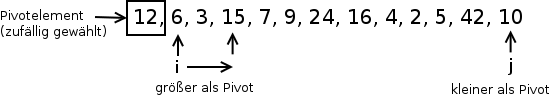
\includegraphics[width=0.6\linewidth]{05/Grafik/img1.png}
\caption{Quicksort}
\end{figure}

$\Rightarrow $ Tausche 15 mit 10 \\
- Bewege Zeiger erneut \\
$\Rightarrow $ Tausche 5 und 24 \\
- Bewege Zeiger erneut \\
$\Rightarrow $ Tausche 16 und 2 \\
- Bewege Zeiger erneut \\
$\Rightarrow $ i wird größer als j $\Rightarrow $  Abbruch (tausche Pivotelement mit letztem Element in Teilliste 1) \\
$\Rightarrow $ es ergeben sich zwei Teillisten \\

4, 6, 3, 10, 7, 9 , 5, 2 |12| 16, 24, 42, 15
\paragraph{best-case}  $T(n) = 2 T \left(\frac{n}{2} \right) + n = \Theta(n \log n) $
\paragraph{worst-case}  $T(n) = T(n-1) + n = \Theta(n^2) $
